\documentclass[a4paper,10pt]{report}
\usepackage{Cours}
\usepackage{delarray}
\usepackage{fancybox}
\newcommand{\Sum}[2]{\ensuremath{\textstyle{\sum\limits_{#1}^{#2}}}}
\newcommand{\Int}[2]{\ensuremath{\mathchoice%
	{{\displaystyle\int_{#1}^{#2}}}
	{{\displaystyle\int_{#1}^{#2}}}
	{\int_{#1}^{#2}}
	{\int_{#1}^{#2}}
	}}
\usepackage{pstricks-add}



\begin{document}
% \everymath{\displaystyle}

\maketitle{Chapitre 19}{Calcul différentiel}

\noindent Dans tout le chapitre, $p$ sera un entier naturel non nul.

\medskip

\noindent Le but de ce chapitre est l'étude de fonctions de $\mathbb{R}^p$ dans $\mathbb{R}$. Par exemple, posons :
$$ f : (x,y,z) \in \mathbb{R}^3 \rightarrow xe^y\sin(z) $$ 
La fonction $f$ est continue (d'après le cours sur espaces vectoriels normés) mais que peut-on dire plus ? On sait étudier plus précisément les fonctions de $\mathbb{R}$ dans $\mathbb{R}$ en utilisant la notion de dérivabilité : le but est donc de généraliser cette notion.

\medskip

\noindent Dans tout le chapitre, $U$ sera un \textit{ouvert} de $\mathbb{R}^p$, $\Vert \cdot \Vert$ sera une norme sur $\mathbb{R}^p$ et $\mathcal{B}= (e_1, \ldots, e_p)$ la base canonique de $\mathbb{R}^p$.

\section{Fonctions de classe $\mathcal{C}^1$}
\subsection{Dérivées partielles}
\begin{defin} Soient $f : U \rightarrow \mathbb{R}$, $a =(a_1, \ldots, a_p) \in U$ et $i \in \Interv{1}{p}$. On dit que $f$ admet une \textit{dérivée partielle} en $a$ par rapport à la $i$-ème variable si la fonction :
$$ t \mapsto f(a_1, \ldots, a_{i-1}, t, a_{i+1}, \ldots, a_p) $$
est dérivable en $a_i$. Lorsque c'est le cas, on note cette dérivée $\partial_i f(a)$ ou $\dfrac{\partial f}{\partial x_i }(a)\cdot$
\end{defin}



\begin{ex} Reprenons l'exemple de début de chapitre : 
 $$f : (x,y,z) \in \mathbb{R}^3 \rightarrow xe^y\sin(z)$$
Soit $a=(1,0,1)$. La fonction :
$$ t \mapsto f(1,t,1) = e^t \sin(1)$$
est dérivable en $0$ et sa dérivée vaut $\sin(1)$. Ainsi $\partial_2 f((1,0,1))=\sin(1)$.
\end{ex}

\medskip

\begin{rem} Si $f$ est définie \og par morceaux \fg, on revient à la définition de dérivabilité. En particulier si $f$ est définie sur un ouvert $U$ de $\mathbb{R}^2$ et si $(a,b) \in U$, on pourra étudier les limites de 
$$ \dfrac{f(a+h,b)-f(a,b)}{h} \; \hbox{ et } \; \dfrac{f(a,b+h)-f(a,b)}{h}$$
quand $h$ tend vers $0$ pour l'existence des dérivées partielles en $(a,b)$. On généralise pour une fonction définie sur un ouvert de $\mathbb{R}^p$.
\end{rem}

\medskip

\begin{ex} Soit $f : \mathbb{R}^2 \rightarrow \mathbb{R}$ l'application définie par :
$$ f((x,y)) = \left\lbrace \begin{array}{ccl}
\dfrac{x^3-y^3}{x^2+y^2} & \hbox{ si } (x,y) \neq (0,0) \\[0.3cm]
0 & \hbox{ si } (x,y)=(0,0) \\
\end{array}\right.$$
Étudions l'existence des deux dérivées partielles de $f$ en $(0,0)$.

% Remarquons que la fonction est définie \og par morceaux \fg : on revient donc à la définition pour étudier la dérivabilité.
%
%\begin{itemize}
%\item Pour tout réel $t \neq 0$, on a :
%$$ \frac{f((t,0))-f((0,0))}{t} = 1 \underset{t \rightarrow 0}{\rightarrow} 1 $$
%Donc $f$ admet une dérivée partielle en $(0,0)$ par rapport à la première variable et l'on a :
%$$ \partial_1 f((0,0)) = 1 $$
%\item Pour tout réel $t \neq 0$, on a :
%$$ \frac{f((0,t))-f((0,0))}{t} = -1 \underset{t \rightarrow 0}{\rightarrow} 1 $$
%Donc $f$ admet une dérivée partielle en $(0,0)$ par rapport à la seconde variable et l'on a :
%$$ \partial_2 f((0,0)) = -1 $$
%\end{itemize}

\vspace{8cm}
\end{ex}

\newpage

$\phantom{test}$

\vspace{4cm}

\begin{rems}
\item L'hypothèse que $\Omega$ soit un ouvert est importante : pour étudier la dérivabilité de 
$$  t \mapsto f(a_1, \ldots, a_{i-1}, t, a_{i+1}, \ldots, a_p) $$
en $a=(a_1, \ldots, a_n)$, on souhaite que si $t$ soit proche de $a_i$ alors $(a_1, \ldots, a_{i-1}, t, a_{i+1}, \ldots, a_p)$ appartienne toujours à $\Omega$. En fait, la $i$-ième application partielle est définie sur l'ensemble suivant :
$$ \lbrace t \in \mathbb{R} \, \vert \, (a_1, \ldots, a_{i-1}, t, a_{i+1}, \ldots, a_p) \in U \rbrace$$
\item Si $p=2$, on note généralement $\dfrac{\partial f}{\partial x}(a)$ au lieu de $\partial_1 f(a)$ et $\dfrac{\partial f}{\partial y}(a)$ au lieu de $\partial_2 f(a)$.
\end{rems}

\begin{defin} Si $f : U \rightarrow \mathbb{R}$ admet une dérivée partielle par rapport à la $i$-ème variable en tout point de $U$ alors la fonction définie sur $U$ et à valeurs dans $\mathbb{R}$ définie par :
$$ a \mapsto \partial_i f(a)$$
est appelée \textit{dérivée partielle} de $f$ par rapport à la $i$-ième variable.
\end{defin}

\subsection{Différentielle}

\begin{defin} Une fonction $f : U \rightarrow \mathbb{R}$ est dite de \textit{classe} $\mathcal{C}^1$ sur $U$ si $f$ admet des dérivées partielles sur $U$, par rapport à toutes ses variables, et si celles-ci sont continues sur $U$.
\end{defin}

\begin{thm} Soit $f: U \rightarrow \mathbb{R}$ une fonction de classe $\mathcal{C}^1$. Alors $f$ admet en tout point $a \in U$ le développement limité à l'ordre $1$ suivant :
$$ f(a+h) = f(a) + \dfrac{\partial f}{\partial x_1}(a) h_1 + \dfrac{\partial f}{\partial x_2}(a) h_2 + \cdots + \dfrac{\partial f}{\partial x_p}(a) h_p + \Vert h \Vert \varepsilon(h)$$
où $\varepsilon : \mathbb{R}^p \rightarrow \mathbb{R}$ a pour limite $0$ en $(0, 0, \ldots,0)$.
\end{thm}

\begin{rem} On peut aussi écrire :
$$ f(a+h) = f(a) + \dfrac{\partial f}{\partial x_1}(a) h_1 + \dfrac{\partial f}{\partial x_2}(a) h_2 + \cdots + \dfrac{\partial f}{\partial x_p}(a) h_p + o(\Vert h \Vert)$$
\end{rem}

\begin{defin} Soient $f : U \rightarrow \mathbb{R}$ une fonction de classe $\mathcal{C}^1$ et $a \in U$. On appelle \textit{différentielle} de $f$ en $a$ la forme linéaire suivante :
$$ \begin{array}{cccll}
\textrm{d}f(a) & : & \mathbb{R}^p & \rightarrow & \mathbb{R} \\
& & (h_1, \ldots, h_p) & \mapsto & \dfrac{\partial f}{\partial x_1}(a) h_1 + \dfrac{\partial f}{\partial x_2}(a) h_2 + \cdots + \dfrac{\partial f}{\partial x_p}(a) h_p \\
\end{array}$$
L'image de $h \in \mathbb{R}^p$ par $\textrm{d}f(a)$ est usuellement notée $\textrm{d}f(a) \cdot h$ au lieu de $\textrm{d}f(a)(h)$.
\end{defin}

\newpage

\begin{rems}
\item La fonction $f$ est définie sur $U$ et $\textrm{d}f$ est définie sur $\mathbb{R}^p$ tout entier.
\item Si $f : U \rightarrow \mathbb{R}$ est de classe $\mathcal{C}^1$ sur $U$ on a donc pour tout $a \in U$,
$$ f(a+h)=f(a) + \textrm{d}f(a) \cdot h + o (\Vert h \Vert)$$
Remarquons que si $f : I \rightarrow\mathbb{R}$ est de classe $\mathcal{C}^1$ sur $I$, un intervalle de $\mathbb{R}$, alors pour tout $a \in I$,
$$ f(a+h)=f(a) + h f'(a) + o(h)$$
Dans le cas de plusieurs variables, le terme 
$$   \textrm{d}f(a) \cdot h = \dfrac{\partial f}{\partial x_1}(a) h_1 + \dfrac{\partial f}{\partial x_2}(a) h_2 + \cdots + \dfrac{\partial f}{\partial x_p}(a) h_p$$
généralise $f'(a)h$ en prenant compte des accroissements de $f$ dans toutes les directions.
\end{rems}

\begin{cor} Soient $I$ un intervalle de $\mathbb{R}$ et $f : I \rightarrow \mathbb{R}$ une fonction de classe $\mathcal{C}^1$. Alors pour tout $a \in I$, 
$$\textrm{d}f(a) : h \in \mathbb{R} \rightarrow f'(a)h$$
\end{cor}

\begin{prop} Si $f$ est de classe $\mathcal{C}^1$ sur $U$ alors $f$ est continue sur $U$.
\end{prop}

\begin{preuve} Évident avec le développement limité de $f$ en $a$ et le fait que $\textrm{d}f(a)$ soit continue.
\end{preuve}

\subsection{Gradient}

\begin{defin} Soient $f : U \rightarrow \mathbb{R}$ une fonction de classe $\mathcal{C}^1$ et $a \in U$. Le vecteur :
$$ \nabla f(a) = \left(\dfrac{\partial f}{\partial x_1}(a), \ldots,   \dfrac{\partial f}{\partial x_p}(a) \right) $$
est appelé \textit{gradient} de $f$ en $a$. La fonction $\nabla f : U \rightarrow \mathbb{R}^p$ est appelée \textit{gradient} de $f$.
\end{defin}

\begin{rem} En utilisant le produit scalaire usuel sur $\mathbb{R}^p$, on a pour tout $h \in \mathbb{R}^p$,
$$ \textrm{d}f(a) \cdot h = < \nabla f(a),h>$$
\end{rem}
\subsection{Quelques propriétés}

\begin{prop} 
\begin{itemize}
\item Toute fonction polynômiale définie sur un ouvert est de classe $\mathcal{C}^1$ sur celui-ci.
\item Toute application linéaire de $\mathbb{R}^p$ dans $\mathbb{R}$ est de classe $\mathcal{C}^1$.
\item Toute fonction rationnelle définie sur un ouvert dont le dénominateur ne s'annule pas est de $\mathcal{C}^1$ sur cet ouvert.
\end{itemize}
\end{prop}

\begin{prop} Soient $f : U \rightarrow \mathbb{R}$ et $g :  U \rightarrow \mathbb{R}$ deux fonctions de classe $\mathcal{C}^1$ et $\lambda \in \mathbb{R}$. Alors $\lambda f+g$ est de classe $\mathcal{C}^1$ sur $U$ et pour tout $a \in U$,
$$ \textrm{d}(\lambda f + g)(a) = \lambda \textrm{d}f(a)+\textrm{d}g(a)$$
et en particulier :
$$ \forall i \in \Interv{1}{p}, \; \dfrac{\partial (\lambda f +g)}{\partial x_i}(a) = \lambda \dfrac{\partial f}{\partial x_i}(a) +  \dfrac{\partial g}{\partial x_i}(a)$$
\end{prop}

\begin{rem} En particulier, l'ensemble $\mathcal{C}^1(U, \mathbb{R})$ est un $\mathbb{R}$-espace vectoriel.
\end{rem}

\begin{prop} Soient $f : U \rightarrow \mathbb{R}$ et $g :  U \rightarrow \mathbb{R}$ deux fonctions de classe $\mathcal{C}^1$. Alors $fg$ est de classe $\mathcal{C}^1$ sur $U$ et pour tout $a \in U$,
$$ \textrm{d}(fg)(a) =\textrm{d}f(a)g(a) + f(a) \textrm{d}g(a)$$
et en particulier :
$$ \forall i \in \Interv{1}{p}, \; \dfrac{\partial (fg)}{\partial x_i}(a) = \dfrac{\partial f}{\partial x_i}(a) g(a) +f(a)  \dfrac{\partial g}{\partial x_i}(a)$$
\end{prop}

\begin{prop} Soient $f : U \rightarrow \mathbb{R}^*$ une fonction de classe $\mathcal{C}^1$. Alors $\dfrac{1}{f}$ est de classe $\mathcal{C}^1$ sur $U$ et pour tout $a \in U$,
$$\textrm{d}(1/f)(a) = - \dfrac{1}{f(a)^2} \textrm{d}f(a)$$
et en particulier :
$$ \forall i \in \Interv{1}{p}, \; \dfrac{\partial (1/f)}{\partial x_i}(a) = - \dfrac{1}{f(a)^2} \dfrac{\partial f }{\partial x_i}(a)$$
\end{prop}



\section{Règle de la chaîne}
\subsection{Propriété et conséquences}
\begin{thm}[Règle de la chaîne] Soient $I$ un intervalle de $\mathbb{R}$ et $x_1$, $x_2$, $\ldots$, $x_p$ des fonctions de classe $\mathcal{C}^1$ sur $I$ et à valeurs dans $\mathbb{R}$. Soit $f : U \rightarrow \mathbb{R}$ une fonction de classe $\mathcal{C}^1$. On suppose que pour tout $t \in I$,
$$ (x_1(t), \ldots, x_p(t)) \in U$$
Alors la fonction $g : I \rightarrow \mathbb{R}$ définie pour tout $t \in I$ par :
$$ g(t)=f(x_1(t), \ldots, x_p(t))$$
est définie et de classe $\mathcal{C}^1$ sur $I$ et pour tout $t \in I$,
$$ g'(t) = \sum_{i=1}^p x_i'(t) \dfrac{\partial f}{\partial x_i}(x_1(t), \ldots, x_p(t))$$
\end{thm}

\medskip

\begin{att} $\dfrac{\partial f}{\partial x_i}$ est une notation pour la dérivée partielle par rapport à la $i$-ième variable et n'a rien à voir avec la fonction $x_i$.
\end{att}

\medskip

\begin{ex} Soient $f : \mathbb{R}^2 \rightarrow \mathbb{R}$ une fonction de classe $\mathcal{C}^1$ et $r \in \mathbb{R}$. On suppose que $f$ est homogène de degré $r$, c'est-à-dire :
$$ \forall (x,y) \in \mathbb{R}^2, \; \forall t >0, \; f(tx,ty) = t^r f(x,y)$$
Montrons que pour tout $(x,y) \in \mathbb{R}^2$,
$$ x \dfrac{\partial f}{\partial x}(x,y) + y \dfrac{\partial f}{\partial y}(x,y) =r f(x,y)$$

\vspace{5cm}
\end{ex}


\newpage

\begin{rem} La formule précédente s'écrit :
$$ \forall t \in I, \; g'(t) =\textrm{d}f(\gamma(t)) \cdot \gamma'(t)$$
où $\gamma =(x_1, \ldots, x_p)$. La fonction $g'$ représente la \textit{dérivée de $f$ le long de l'arc} $(I, \gamma)$.
\end{rem}

\medskip

\noindent On s'intéresse maintenant à la situation suivante : 

$$ \begin{array}{ccccccc}
V \subset \mathbb{R}^2 & \overset{(x,y)}{\rightarrow} & U \subset \mathbb{R}^2 & \overset{f}{\rightarrow} & \mathbb{R} \\
(u,v) & \mapsto & (x(u,v),y(u,v)) & \mapsto & f(x(u,v),y(u,v)) \\
\end{array}$$

\begin{prop} Soient $V$ un ouvert de $\mathbb{R}^2$, $x$ et $y$ deux fonctions de classe $\mathcal{C}^1$ sur $V$ et à valeurs réelles. Soient $U$ un ouvert de $\mathbb{R}^2$ et $f : U \rightarrow \mathbb{R}$ de classe $\mathcal{C}^1$ sur $U$. On suppose que pour tout $(u,v) \in V$,
$$ (x(u,v),y(u,v)) \in U$$
Alors la fonction $g : V \rightarrow \mathbb{R}$ définie pour tout $(u,v) \in V$ par 
$$ g(u,v) = f(x(u,v),y(u,v))$$
est de classe $\mathcal{C}^1$ sur $V$ et pour tout $(u,v) \in V$,
\begin{align*}
\dfrac{\partial g}{\partial u} (u,v) = \dfrac{\partial f}{\partial x}(x(u,v),y(u,v)) \dfrac{\partial x}{\partial u}(u,v) + \dfrac{\partial f}{\partial y}(x(u,v),y(u,v)) \dfrac{\partial y}{\partial u}(u,v) \\
\dfrac{\partial g}{\partial v} (u,v) = \dfrac{\partial f}{\partial x}(x(u,v),y(u,v)) \dfrac{\partial x}{\partial v}(u,v) + \dfrac{\partial f}{\partial y}(x(u,v),y(u,v)) \dfrac{\partial y}{\partial v}(u,v) \\
\end{align*}
\end{prop}

\noindent \textbf{Exemple fondamental : passage en coordonnées polaires.}

\noindent Soit $(x,y) \in \mathbb{R}^2$. Il existe alors $r \in \mathbb{R}_+$ et $\theta \in \mathbb{R}$ tels que :
$$ (x,y) = (r \cos(\theta), r \sin(\theta))$$
On appelle $r$ et $\theta$ les \textit{coordonnées polaires} de $(x,y)$. Il n'y a évidemment pas unicité de ces coordonnées : Si $(x,y)=(0,0)$, $r=0$ et tout réel $\theta$ convient et si $(x,y)$ est différent de $(0,0)$, $\theta$ est \og défini \fg modulo $2\pi$. 

\medskip

\noindent Soit $f : \mathbb{R}^2 \rightarrow \mathbb{R}$ une fonction de classe $\mathcal{C}^1$. On pose pour tout $(r, \theta) \in \mathbb{R}^2$,
$$ g(r, \theta)= f(r \cos(\theta), r \sin(\theta))$$
Justifions que $g$ est $\mathcal{C}^1$ sur $\mathbb{R}^2$ et déterminons ses dérivées partielles.

\vspace{7cm}

\newpage

\subsection{Fonctions constantes}

\begin{prop} Soit $f : U \rightarrow \mathbb{R}$ une fonction de classe $\mathcal{C}^1$ sur $U$ un ouvert \textit{convexe}. Alors $f$ est constante si et seulement si pour tout $i \in \Interv{1}{p}$, $\dfrac{\partial f}{\partial x_i}=0$.
\end{prop}

\begin{prop} Soit $f : U \rightarrow \mathbb{R}$ une fonction de classe $\mathcal{C}^1$ sur $U$ un ouvert \textit{convexe} avec $p \geq 2$. Supposons que :
$$ \dfrac{\partial f }{\partial x_1} = 0$$
Alors la fonction $f$ ne \og dépend pas \fg{} de sa première variable : il existe un ouvert convexe $Z$ de $\mathbb{R}^{p-1}$ et une fonction $g : Z \rightarrow \mathbb{R}$ tel que pour tout $(x_1, \ldots, x_p) \in U$, $(x_2, \ldots,x_p) \in Z$ et 
$$f(x_1, \ldots, x_p) = g(x_2, \ldots, x_p) $$
\end{prop}

\begin{rem} On généralise évidemment aux autres variables.
\end{rem}

\section{Problèmes d'extrema}
\noindent Dans toute cette section, on considère une fonction $f : U \rightarrow \mathbb{R}$ où $U$ est un ouvert de $\mathbb{R}^p$.

\begin{defin} Soit $a \in U$.
\begin{itemize}
\item On dit que $f$ admet un \textit{minimum local} en $a$ si et il existe $r >0$ tel que $B(a,r) \subset U$ et tel que pour tout $x \in B(a,r)$, $f(x) \geq f(a)$.
\item On dit que $f$ admet un \textit{minimum global} en $a$ si pour tout $x \in U$, $f(x) \geq f(a)$.
\end{itemize}
\end{defin}

\begin{rem} On définit de même la notion de maximum local et maximum global.
\end{rem}

\begin{defin}
Soient $f : U \rightarrow \mathbb{R}$ une fonction de classe $\mathcal{C}^1$ et $a \in U$. On dit que $a$ est un \textit{point critique} de $f$ si $\nabla f (a)$ est le vecteur nul, c'est-à-dire :
$$ \forall i \in \Interv{1}{p}, \; \dfrac{\partial f}{\partial x_i}(a)= 0 $$
\end{defin}

\begin{prop}
Si $f : U \rightarrow \mathbb{R}$ est de classe $\mathcal{C}^1$ sur $U$ et admet un extremum local en $a \in U$ alors $a$ est un point critique de $f$.
\end{prop}

\begin{preuve}

\vspace{5cm}
\end{preuve}

\newpage
\begin{rem}
Attention c'est une condition nécessaire ! Considérons par exemple :
$$ \begin{array}{cccll}
f& : & \mathbb{R} & \rightarrow & \mathbb{R} \\
& & (x,y) & \mapsto & x^2+y^2-4xy 
\end{array}$$

\vspace{5cm}
\end{rem}

\medskip

\begin{center}
\textbf{Comment étudier l'existence d'un extremum local ?}
\end{center}

\medskip

\begin{itemize}
\item Si $a \in U$ est un point critique de $f$, on peut étudier le signe de $f(x)-f(a)$ pour $x$ proche de $a$. Si le signe est constant sur un voisinage de $a$ : $f$ admet un extremum local. Si on trouve des vecteurs $x$ arbitrairement proches de $a$ tels que $f(x)-f(a)>0$ et $f(x)-f(a)<0$ alors $f$ n'admet pas d'extremum local en $a$.
\item Si $f$ est continue sur un compact (fermé borné) $K$ alors on sait que $f$ admet un maximum et un minimum global sur $K$. Alors si $f$ est de classe $\mathcal{C}^1$ sur l'intérieur de $K$, les points où $f$ admet ces extrema sont soit des points critiques de $f$ sur l'intérieur de $K$, soit se situent sur la frontière.
\end{itemize}

\medskip

\begin{ex} Justifions l'existence et déterminons le maximum de la fonction $f$ définie sur l'ensemble $K=\lbrace (x,y) \in \mathbb{R}^2  \, \vert \, x \geq 0, \,  y \geq 0 \hbox{ et } x+y \leq 1\rbrace$ par : 
  \[
  f(x,y) = xy(1-x-y)
  \]





%Justifions l'existence et déterminons le maximum de la fonction $f$ définie sur $K=[0,1]^2$ par : 
%  \[
%  f(x,y) = \frac{x + y}{(1 + x^{2})(1 + y^{2})}
%  \]
  
  \vspace{10cm}
\end{ex}

\newpage

\section{Dérivées partielles d'ordre deux}

\begin{defin} Soit $f : U \rightarrow \mathbb{R}$ une fonction. On dit que $f$ est de classe $\mathcal{C}^2$ sur $U$ si $f$ est de classe $\mathcal{C}^1$ sur $U$ et si les dérivées partielles de $f$ sont $\mathcal{C}^1$ sur $U$.
\end{defin}

\noindent Pour tout $(i,j) \in \Interv{1}{p}^2$, $\dfrac{\partial f}{\partial x_i} \left( \dfrac{\partial f}{\partial x_j} \right)$ est généralement notée $\dis \dfrac{\partial^2 f}{\partial x_i \partial x_j}$ ou $\partial^2_{i,j} f$.

\noindent De plus si $i=j$, on écrit $\dfrac{\partial^2 f}{\partial x_i^2}$ au lieu de $\dis \dfrac{\partial^2 f}{\partial x_i \partial x_i}\cdot$

\medskip


\begin{rem} Les résultats concernant les opérations sur les fonctions de classe $\mathcal{C}^1$, les propriétés des fonctions polynômiales, applications linéaires, fractions rationnelles, se généralisent aux fonctions de classes $\mathcal{C}^2$.
\end{rem}

\begin{thm}[Schwarz]
Si $f$ est de classe $\mathcal{C}^2$ sur $U$ alors pour tout $(i,j) \in \Interv{1}{p}^2$,
$$ \dfrac{\partial^2 f}{\partial x_i \partial x_j} = \dfrac{\partial^2 f}{\partial x_j \partial x_i}$$
\end{thm}

\begin{ex} Soit :
$$\begin{array}{cccll}
f& : & \mathbb{R} & \rightarrow & \mathbb{R} \\
& & (x,y) & \mapsto & x^2+y^3-4xy 
\end{array}$$

\vspace{5cm}
\end{ex}

\section{Courbes et surfaces}
\noindent Dans le chapitre lié aux arcs paramétrés, nous avons étudié les arcs paramétrés plans de la forme $(x,y)$. Nous allons maintenant donner des résultats concernant des courbes ou des surfaces définies par une équation cartésienne de la forme $f(x,y)=0$ ou $f(x,y,z)=0$ où $f$ est une fonction définie sur un ouvert de $\mathbb{R}^2$ ou $\mathbb{R}^3$ à valeurs dans $\mathbb{R}$.

\medskip

\noindent Dans cette section, on considère $\mathbb{R}^2$ ou $\mathbb{R}^3$ muni du produit scalaire usuel.

\subsection{Courbes définies par une équation cartésienne}
\medskip

\noindent On appelle courbe du plan \textit{définie par une équation cartésienne} tout ensemble $\mathcal{C}$ de $\mathbb{R}^2$ défini par :
$$ \mathcal{C} = \lbrace (x,y) \in U \, \vert \, f(x,y)=0 \rbrace$$
où $f : U \rightarrow \mathbb{R}$ est une fonction de classe $\mathcal{C}^1$ définie sur un ouvert $U$ de $\mathbb{R}^2$.

\medskip

\begin{exems}
\item Considérons $\mathcal{C}$ le cercle unité de $\mathbb{R}^2$.

\vspace{5cm}
\item Soit $g : I \rightarrow \mathbb{R}$ une fonction de classe $\mathcal{C}^1$ sur un intervalle non vide $I$ de $\mathbb{R}$.

\vspace{5cm}
\end{exems}

\begin{defin} Soit $f : U \rightarrow \mathbb{R}$ une fonction de classe $\mathcal{C}^1$ et $\mathcal{C}$ la courbe définie par :
$$ \mathcal{C} = \lbrace (x,y) \in U \, \vert \, f(x,y)=0 \rbrace$$
\noindent On appelle \textit{point régulier} de $\mathcal{C}$ tout point $(x_0,y_0) \in \mathcal{C}$ tel que :
$$ \nabla f(x_0,y_0) \neq (0,0)$$
\end{defin}
\noindent Ainsi, un point régulier de $\mathcal{C}$ est un point de cette courbe qui n'est pas un point critique de $f$.

\begin{thm} Gardons les notations de la définition précédente. Soit $(x_0,y_0)$ un point régulier de $\mathcal{C}$. Alors il existe $r>0$, $\eta>0$ et $\gamma : ]- \eta, \eta[ \rightarrow U$ de classe $\mathcal{C}^1$ tels que :
\begin{itemize}
\item $\gamma(0)= (x_0,y_0)$.
\item $(]-\eta,\eta[, \gamma)$ est un arc paramétré régulier où $\gamma$ est injective.
\item Pour tout $(x,y) \in B((x_0,y_0),r)$, on a :
$$ f(x,y)=0 \Longleftrightarrow \exists t \in ]- \eta, \eta[, \; (x,y)=\gamma(t)$$
\end{itemize}
On appelle $(]-\eta,\eta[, \gamma)$ un \textit{paramétrage local} de $\mathcal{C}$ au voisinage de $(x_0,y_0)$.
\end{thm}

\medskip

\noindent Autrement dit, au voisinage d'un point régulier, une courbe définie par une équation cartésienne (donc de manière implicite) peut être explicitée comme l'image d'un arc paramétré ($x$ et $y$ s'expriment en fonction du paramètre $t$).

\medskip

\begin{defip} Soit $f : U \rightarrow \mathbb{R}$ de classe $\mathcal{C}^1$ sur $U$ et $\mathcal{C}$ la courbe de $\mathbb{R}^2$ définie par $f(x,y)=0$. Soit $(x_0,y_0)$ un point régulier de $\mathcal{C}$.
\begin{itemize}
\item La courbe $\mathcal{C}$ possède une tangente en $(x_0,y_0)$ d'équation :
$$ \dfrac{\partial f}{\partial  x}(x_0,y_0)(x-x_0) + \dfrac{\partial f}{\partial y}(x_0,y_0) (y-y_0)=0$$
\item On appelle \textit{normale} à $\mathcal{C}$ au point $(x_0,y_0)$ la droite passant par $(x_0,y_0)$ et dirigée par :
$$ \nabla f(x_0,y_0) = \left(\dfrac{\partial f}{\partial  x}(x_0,y_0), \dfrac{\partial f}{\partial  y}(x_0,y_0) \right)$$
On dit que $ \nabla f(x_0,y_0)$ est orthogonal à $\mathcal{C}$ au point $(x_0,y_0)$.
\end{itemize}
\end{defip}

%\noindent \textbf{Idée de la preuve}
%
%\vspace{7cm}
%
%
%\newpage
%
%$\phantom{test}$
%
%\vspace{4cm}

\begin{ex} Soit $\mathcal{C}$ la courbe d'équation :
$$ x^3+3y^2+6xy+4=0$$
Déterminons les points réguliers de $\mathcal{C}$ et l'équation de la tangente à $\mathcal{C}$ en ces points.

\newpage

$\phantom{}$
\vspace{10cm}
\end{ex}

\begin{defin} Soient $f : U \rightarrow \mathbb{R}$ et $\lambda \in \mathbb{R}$. On appelle \textit{ligne de niveau} $\lambda$ de $f$ le sous-ensemble de $U$ d'équation $f(x,y)=\lambda$.
\end{defin}

\begin{center}
\textbf{Exemples de lignes de niveaux : $z=f(x,y)$}
\end{center}

\begin{center}
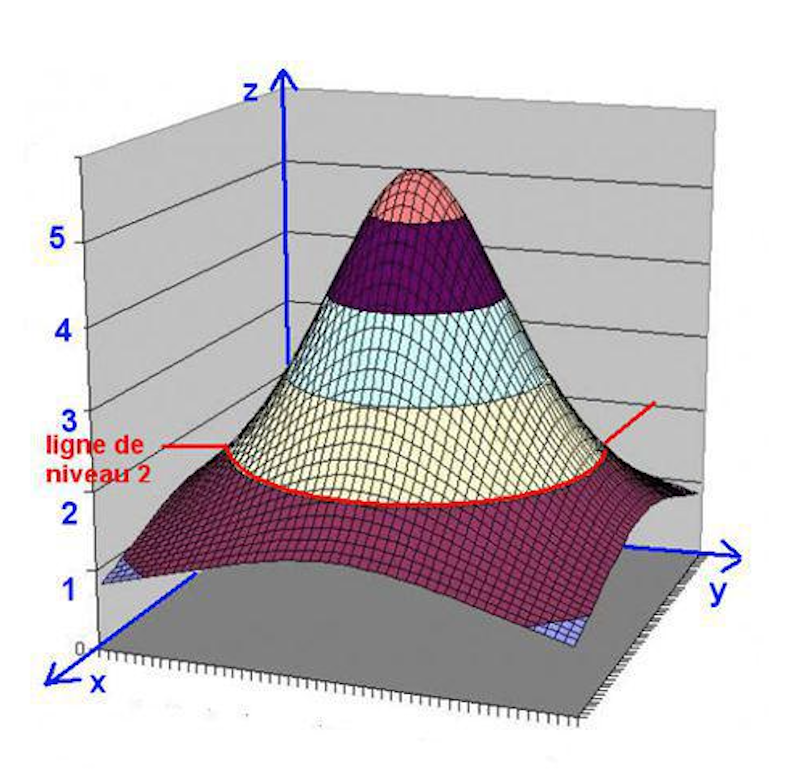
\includegraphics[scale=0.5]{niv}
\end{center}

\begin{prop} Soient $f : U \rightarrow \mathbb{R}$ une fonction de classe $\mathcal{C}^1$ et $\lambda \in \mathbb{R}$.

\noindent Soit $(x_0,y_0)$ un point régulier de la ligne de niveau $\lambda$ de $f$, c'est-à-dire : $f(x_0,y_0)=\lambda$ et $\nabla f (x_0,y_0) \neq (0,0)$. Alors $\nabla  f (x_0,y_0)$ est orthogonal  à la ligne de niveau $\lambda$ de $f$ et orienté dans le sens des valeurs croissantes de $f$ : il existe $\delta >0$ tel que 
$$ t \mapsto f((x_0,y_0) + t \nabla  f (x_0,y_0))$$
soit strictement croissante sur $]-\delta, \delta[$.
\end{prop}

\begin{ex} Étudions les lignes de niveaux de $f : (x,y) \mapsto x^2+y^2$.

\vspace{6cm}
\end{ex}



\subsection{Surfaces définies par une équation cartésienne}
\medskip

\noindent On appelle surface de l'espace \textit{définie par une équation cartésienne} tout ensemble $\mathcal{S}$ de $\mathbb{R}^3$ défini par :
$$ \mathcal{S} = \lbrace (x,y,z) \in U \, \vert \, f(x,y,z)=0 \rbrace$$
où $f : S \rightarrow \mathbb{R}$ est une fonction de classe $\mathcal{C}^1$ définie sur un ouvert $U$ de $\mathbb{R}^3$.

\medskip

\begin{exems}
\item Considérons $\mathcal{S}$ la sphère unité de $\mathbb{R}^3$.

\vspace{5cm}
\item Soit $g : Z \rightarrow \mathbb{R}$ une fonction de classe $\mathcal{C}^1$ sur un ouvert $Z$ de $\mathbb{R}^2$. La surface représentative $\mathcal{S}_g$ de $g$ est définie par les triplets $(x,y,z)$ où $(x,y) \in Z$ et $z \in \mathbb{R}$ tels que $z=g(x,y)$. Cette égalité est équivalente à $f(x,y,z) =0$ où :
$$ f : (x,y,z) \mapsto z-g(x,y) $$
\end{exems}

\begin{defin} Soient $f : U \rightarrow \mathbb{R}$ une fonction de classe $\mathcal{C}^1$ et $\mathcal{S}$ la surface définie par :
$$ \mathcal{S} = \lbrace (x,y,z) \in U \, \vert \, f(x,y,z)=0 \rbrace$$
\noindent On appelle \textit{point régulier} de $\mathcal{C}$ tout point $(x_0,y_0,z_0) \in \mathcal{S}$ tel que :
$$ \nabla f(x_0,y_0,z_0) \neq (0,0,0)$$
\end{defin}
\noindent Ainsi, un point régulier de $\mathcal{S}$ est un point de cette surface qui n'est pas un point critique de $f$.

\begin{defin} Soient $f : U \rightarrow \mathbb{R}$ de classe $\mathcal{C}^1$ sur $U$ et $\mathcal{S}$ la surface de $\mathbb{R}^3$ définie par $f(x,y,z)=0$. Soit $(x_0,y_0,z_0)$ un point régulier de $\mathcal{S}$.

\noindent On appelle \textit{plan tangent} à $\mathcal{S}$ en $(x_0,y_0,z_0)$ le plan orthogonal à $\nabla f(x_0,y_0,z_0)$ et passant par $(x_0,y_0,z_0)$. C'est donc le plan d'équation :
$$ \dfrac{\partial f}{\partial x}(x_0,y_0,z_0) (x-x_0) +  \dfrac{\partial f}{\partial y}(x_0,y_0,z_0) (y-y_0) +  \dfrac{\partial f}{\partial z}(x_0,y_0,z_0) (z-z_0) = 0$$
\end{defin}

\medskip

\begin{center}
\textbf{Exemple de plan tangent}
\end{center}

\begin{center}
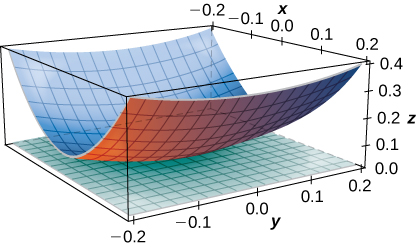
\includegraphics[scale=1]{tan}
\end{center}

\begin{defin} Soient $f : U \rightarrow \mathbb{R}$ de classe $\mathcal{C}^1$ et $\mathcal{S}$ la surface définie par $f(x,y,z)=0$. On appelle \textit{courbe tracée sur la surface} $\mathcal{S}$ tout arc paramétré $(I, \gamma)$ où $I$ est un intervalle non vide de $\mathbb{R}$ et $ \gamma =(x,y,z) : I \rightarrow \mathbb{R}^3$ vérifie :
$$ \forall t \in I, \; (x(t),y(t),z(t)) \in \mathcal{S}$$
\end{defin}

\begin{prop} Soit $\Gamma$ le support d'une courbe tracée $(I, \gamma)$ sur la surface $\mathcal{S}$ d'équation $f(x,y,z)=0$ où $f : U \rightarrow \mathbb{R}$ est de classe $\mathcal{C}^1$.  Soit $(x_0,y_0,z_0)= \gamma(t_0)  \in \mathcal{S}$ un point régulier de $\mathcal{S}$ et un point régulier de $\Gamma$. Alors la tangente à $\Gamma$ en $\gamma(t_0)$ est contenue dans le plan tangent à $\mathcal{S}$ en $(x_0,y_0,z_0)$.
\end{prop}

%\begin{preuve}
%
%\vspace{7cm}
%\end{preuve}



\section{Exemples de résolution d'équations aux dérivées partielles}
\noindent Dans de nombreux domaines scientifiques, la résolution des équations aux dérivées partielles est primordiale. Si $f : U \rightarrow \mathbb{R}$ est solution d'une équation aux dérivées partielles, il est parfois possible d'utiliser un changement de variable pour déterminer explicitement celle-ci. On souhaite écrire $f(x)$, où $x \in U$, sous la forme :
$$ f(x) = g(\varphi(x)) = g(\varphi_1(x), \ldots, \varphi_p(x))$$
où $\varphi= (\varphi_1, \ldots, \varphi_p)$ est une fonction bijective de $U$ sur un ouvert $V$ de $\mathbb{R}^p$. Dans ce cas, $g = f \circ \varphi^{-1}$. 

\medskip

\noindent L'idée est d'obtenir une équation aux dérivées partielles plus simple vérifiée par $g$ en \og injectant \fg $f= g \circ \varphi^{-1}$ dans l'équation de départ. Évidemment, il est important de vérifier que les fonctions manipulées sont de classe $\mathcal{C}^1$...

\subsection{Équations aux dérivées partielles de base}
\noindent Soit $f$, $g$ et $\varphi$ définies comme précédemment (on suppose ces fonctions de classe $\mathcal{C}^1$ sur leurs ensembles de définition). On note $y_1$ et $y_2$ les variables de la fonction $g$ (on se restreint à ce cas pour l'exemple).

\begin{itemize}
\item Si $\dfrac{\partial g}{\partial y_1} =0$ sur $V$ et si $V$ est convexe alors $g$ ne dépend pas de sa première variable : il existe une fonction $F$ définie sur un intervalle ouvert $I$ de $\mathbb{R}$ tel que pour tout $(y_1,y_2) \in V$, $y_2 \in I$ et $g(y_1,y_2)=F(y_2)$. La réciproque est claire.
\item Si $\dfrac{\partial g}{\partial y_1 \partial y_2} =0$ sur $V$ et si $V$ est convexe alors $\dfrac{\partial g}{\partial y_2}$ ne dépend pas de sa première variable : il existe une fonction $F$ définie sur un intervalle ouvert $I$ de $\mathbb{R}$ tel que pour tout $(y_1,y_2) \in V$, $y_2 \in I$ et :
$$  \dfrac{\partial g}{\partial y_2}(y_1,y_2)=F(y_2)$$
La fonction $(y_1,y_2) \mapsto g(y_1,y_2) - \tilde{F}(y_2)$ où $\tilde{F}$ est une primitive de $F$ sur $I$, a une dérivée partielle par rapport à $y_2$ nulle. En réitérant le procédé précédent, $g$ est de la forme :
$$ g : (y_1,y_2) \mapsto G(y_1)+\tilde{F}(y_2)$$
où $F$ et $G$ sont de classe $\mathcal{C}^2$ sur des intervalles ouverts de $\mathbb{R}$.
\end{itemize}

\medskip

\noindent Dès que $g$ est connue, on obtient $f$...
\subsection{Exemple 1 : transformation affine}
\noindent Résoudre sur $\mathbb{R}^2$ l'équation au dérivées partielles suivante :
$$ \dfrac{\partial f}{\partial x}(x,y) - 3 \dfrac{\partial f}{\partial y}(x,y) = 0$$
en utilisant le changement de variable suivant :
$$ \left\lbrace \begin{array}{ccl}
u & = 2x+y \\
v& = 3x+y \\
\end{array}\right.$$

\newpage

$\phantom{}$
\vspace{10cm}


\subsection{Une remarque sur les coordonnées polaires}
\noindent Fixons $\alpha \in [-\pi,\pi[$. Et considérons l'ensemble $U$ du plan défini comme $\mathbb{R}^2 \setminus D$ où $D$ est la demi-droite formée des points $(x,y)$, dont l'argument de $x+iy$ est égal à $\alpha$, et du point $(0,0)$. Ce qui donne :

\vspace{3cm}

\noindent Dans ce cas, l'application :
$$ \begin{array}{cccll}
\Phi & : & \mathbb{R}_+^{*} \times ]\alpha, \alpha + 2 \pi[ & \rightarrow & U \\
& & (r, \theta) & \mapsto & (r \cos(\theta), r \sin(\theta)) \\
\end{array}$$
est bijective et de classe $\mathcal{C}^1$. L'égalité :
$$ (x,y) = \Phi(r ,\theta)$$ implique que $r= \sqrt{x^2+y^2}$ et 
$$ \cos(\theta) = \dfrac{x}{\sqrt{x^2+y^2}} \hbox{ et } \sin(\theta) = \dfrac{y}{\sqrt{x^2+y^2}} $$

\subsection{Exemple 2 : coordonnées polaires}
\noindent Soit $\mathcal{U} = \mathbb{R}_+^{*} \times \mathbb{R}$. Déterminons toutes les fonctions $f : \mathcal{U} \rightarrow \mathbb{R}$ de classe $\mathcal{C}^1$ telles pour tout $(x,y) \in \mathcal{U}$, $\nabla f (x,y)$ soit colinéaire à $(x,y)$.
\newpage

$\phantom{test}$

\vspace{10cm}

\section{Compléments (sur les fonctions vectorielles)}

\begin{prop}[Composition par une application linéaire]
Soient $p \in \mathbb{N}^*$ et $L : \mathbb{R}^n \rightarrow \mathbb{R}^p$ une application linéaire. Si $f : I \rightarrow \mathbb{R}^n$ est dérivable en $a \in I$ alors $L \circ f : I \rightarrow \mathbb{R}^p$ est dérivable en $a$ et on a :
$$ (L \circ f)'(a) = L (f'(a))$$
\end{prop}

\begin{preuve} Pour tout $x \in I$, $x \neq a$, on a :
$$ \dfrac{(L \circ f)(x) - (L \circ f)(a) }{x-a} = L \left( \frac{f(x)-f(a)}{x-a} \right)$$
par linéarité de $L$. Or $f$ est dérivable en $a$ donc :
$$ \frac{f(x)-f(a)}{x-a} \underset{x \rightarrow a}{\longrightarrow} f'(a)$$
Sachant que $L$ est une application linéaire sur un espace vectoriel de dimension finie, $L$ est donc continue sur $\mathbb{R}^n$ et donc en particulier en $f'(a)$. Ainsi :
$$ L \left( \frac{f(x)-f(a)}{x-a} \right) \underset{x \rightarrow a}{\longrightarrow} L(f'(a))$$
ce qui donne le résultat.
\end{preuve}


\begin{prop}[Composition par une application bilinéaire]
Soient $(m,p) \in (\mathbb{N}^*)^2$ et $B : \mathbb{R}^n \times \mathbb{R}^m \rightarrow \mathbb{R}^p$ une application bilinéaire. Si $f : I \rightarrow \mathbb{R}^n$ et $g : I \rightarrow \mathbb{R}^m$ sont dérivables en $a \in I$ alors $B(f,g):  I \rightarrow \mathbb{R}^p$ est dérivable en $a$ et on a :
$$ B(f,g)'(a)= B(f'(a),g(a))+B(f(a),g'(a))$$
\end{prop}

\begin{preuve}
Pour tout $x \in I$, $x \neq a$, on a par bilinéarité de $B$ :

\begin{align*}
\frac{B(f,g)(x)-B(f,g)(a)}{x-a} & =\frac{B(f(x),g(x))-B(f(a),g(x))+B(f(a),g(x))-B(f(a),g(a))}{x-a} \\
& = B \left( \frac{f(x)-f(a)}{x-a},g(x) \right) + B \left( f(a), \frac{g(x)-g(a)}{x-a} \right) 
\end{align*}
Les fonctions $f$ et $g$ sont dérivables (et donc continues) en $a \in I$ donc :
$$ g(x) \underset{x \rightarrow a}{\longrightarrow} g(a), \; \frac{f(x)-f(a)}{x-a}\underset{x \rightarrow a}{\longrightarrow} f'(a) \et \frac{g(x)-g(a)}{x-a} \underset{x \rightarrow a}{\longrightarrow} g'(a)$$
De plus, $B$ est bilinéaire sur $\mathbb{R}^n \times \mathbb{R}^m$ donc continue sur cet espace donc :
$$ \frac{B(f,g)(x)-B(f,g)(a)}{x-a}   \underset{x \rightarrow a}{\longrightarrow}  B(f'(a),g(a))+ B(f(a),g'(a))$$
ce qui donne le résultat.
\end{preuve}

\begin{cor} Soient $f : I \rightarrow \mathbb{R}^n$ et $\alpha : I \rightarrow \mathbb{R}$ deux fonctions dérivables en $a \in I$. Alors $\alpha f $ est dérivable en $a$ et on a :
$$ (\alpha f)'(a) = \alpha'(a) f(a) + \alpha(a) f'(a)$$
\end{cor}

\begin{preuve} Bilinéarité du produit.
\end{preuve}

\begin{cor} Soient $< \cdot , \cdot>$ un produit scalaire sur $\mathbb{R}^n$ et $f: I \rightarrow \mathbb{R}^n$, $g : I \rightarrow \mathbb{R}^n$ deux fonctions dérivables en $a \in I$. Alors la fonction $<f,g> \, :  I \rightarrow \mathbb{R}$ est dérivable en $a$ et :
$$ <f,g>'(a) = <f'(a),g(a)>+<f(a),g'(a)>$$
\end{cor}

\begin{preuve} $< \cdot , \cdot> \, : \mathbb{R}^n \times \mathbb{R}^n \rightarrow \mathbb{R}$ est bilinéaire.
\end{preuve}
%
%\begin{exa} Rappelons que si $< \cdot , \cdot>$ est un produit scalaire sur $\mathbb{R}^n$, on définit la norme euclidienne par :
%$$ \forall x \in \mathbb{R}^n, \; \Vert x \Vert = \sqrt{<x,x>}$$
%Montrer que si $f : I \rightarrow\mathbb{R}^n$ est dérivable en $a \in I$ alors $\Vert f \Vert^2$ est dérivable en $a$ et on a :
%$$ (\Vert f \Vert^2)'(a) = 2 <f(a),f'(a)>$$
%\end{exa}

%\begin{nota}
%Si $x,y$ sont deux éléments de $\mathbb{R}^2$ et si $\mathcal{B}$ est une base de $\mathbb{R}^2$, on note :
%$$ \textrm{det}_{\mathcal{B}}(x,y) = \textrm{det}(\textrm{Mat}_{\mathcal{B}}(x,y))$$
%\end{nota}

\begin{cor} Soient $\mathcal{B}$ une base de  $\mathbb{R}^2$ et $f: I \rightarrow \mathbb{R}^2$, $g : I \rightarrow \mathbb{R}^2$ deux fonctions dérivables en $a \in I$. Alors la fonction $\textrm{det}_{\mathcal{B}}(f,g)$ est dérivable en $a$ et :
$$ (\textrm{det}_{\mathcal{B}}(f,g))'(a) = \textrm{det}_{\mathcal{B}}(f'(a),g(a)) + \textrm{det}_{\mathcal{B}}(f(a),g'(a))$$
\end{cor}

\begin{preuve} $\textrm{det}_{\mathcal{B}}$ est bilinéaire.
\end{preuve}

\begin{prop}[Composition par une application linéaire]
Soient $p \in \mathbb{N}^*$ et $L : \mathbb{R}^n \rightarrow \mathbb{R}^p$ une application linéaire. 
\begin{itemize}
\item Si $f : I \rightarrow \mathbb{R}^n$ est de classe $\mathcal{C}^k$ sur $I$ alors $L \circ f : I \rightarrow \mathbb{R}^p$ est de classe $\mathcal{C}^k$ sur $I$ et on a pour tout $i \in \Interv{1}{k}$ et tout $a \in I$,
$$ (L \circ f)^{(i)}(a) = L (f^{(i)}(a))$$
\item  Si $f : I \rightarrow \mathbb{R}^n$ est de classe $\mathcal{C}^{\infty}$ sur $I$ alors $L \circ f : I \rightarrow \mathbb{R}^p$ est de classe $\mathcal{C}^{\infty}$ sur $I$ et on a pour tout $i \in \mathbb{N}^*$ et tout $a \in I$,
$$ (L \circ f)^{(i)}(a) = L (f^{(i)}(a))$$
\end{itemize}
\end{prop}

\begin{thm}[formule de Leibniz]
Soient $(m,p) \in (\mathbb{N}^*)^2$ et $B : \mathbb{R}^n \times \mathbb{R}^m \rightarrow \mathbb{R}^p$ une application bilinéaire.  Si $f : I \rightarrow \mathbb{R}^n$ et $g : I \rightarrow \mathbb{R}^m$ sont de classes $\mathcal{C}^k$ sur $I$ alors $B(f,g):  I \rightarrow \mathbb{R}^p$ est de classe $\mathcal{C}^k$ sur $I$ et on a :
$$ B(f,g)^{(k)}(a)=  \sum_{i=0}^{k} \binom{k}{i} B(f^{(i)},g^{(k-i)})$$
\end{thm}

\end{document}
